\documentclass[12pt]{article}
\usepackage{amsmath}
\usepackage{latexsym}
\usepackage{amsfonts}
\usepackage[normalem]{ulem}
\usepackage{array}
\usepackage{amssymb}
\usepackage{graphicx}
\usepackage[backend=biber,
style=numeric,
sorting=none,
isbn=false,
doi=false,
url=false,
]{biblatex}\addbibresource{bibliography.bib}

\usepackage{subfig}
\usepackage{wrapfig}
\usepackage{wasysym}
\usepackage{enumitem}
\usepackage{adjustbox}
\usepackage{ragged2e}
\usepackage[svgnames,table]{xcolor}
\usepackage{tikz}
\usepackage{longtable}
\usepackage{changepage}
\usepackage{setspace}
\usepackage{hhline}
\usepackage{multicol}
\usepackage{tabto}
\usepackage{float}
\usepackage{multirow}
\usepackage{makecell}
\usepackage{fancyhdr}
\usepackage[toc,page]{appendix}
\usepackage[hidelinks]{hyperref}
\usetikzlibrary{shapes.symbols,shapes.geometric,shadows,arrows.meta}
\tikzset{>={Latex[width=1.5mm,length=2mm]}}
\usepackage{flowchart}\usepackage[paperheight=11.0in,paperwidth=8.5in,left=1.0in,right=1.0in,top=1.0in,bottom=1.0in,headheight=1in]{geometry}
\usepackage[utf8]{inputenc}
\usepackage[T1]{fontenc}
\TabPositions{0.5in,1.0in,1.5in,2.0in,2.5in,3.0in,3.5in,4.0in,4.5in,5.0in,5.5in,6.0in,}

\urlstyle{same}


 %%%%%%%%%%%%  Set Depths for Sections  %%%%%%%%%%%%%%

% 1) Section
% 1.1) SubSection
% 1.1.1) SubSubSection
% 1.1.1.1) Paragraph
% 1.1.1.1.1) Subparagraph


\setcounter{tocdepth}{5}
\setcounter{secnumdepth}{5}


 %%%%%%%%%%%%  Set Depths for Nested Lists created by \begin{enumerate}  %%%%%%%%%%%%%%


\setlistdepth{9}
\renewlist{enumerate}{enumerate}{9}
		\setlist[enumerate,1]{label=\arabic*)}
		\setlist[enumerate,2]{label=\alph*)}
		\setlist[enumerate,3]{label=(\roman*)}
		\setlist[enumerate,4]{label=(\arabic*)}
		\setlist[enumerate,5]{label=(\Alph*)}
		\setlist[enumerate,6]{label=(\Roman*)}
		\setlist[enumerate,7]{label=\arabic*}
		\setlist[enumerate,8]{label=\alph*}
		\setlist[enumerate,9]{label=\roman*}

\renewlist{itemize}{itemize}{9}
		\setlist[itemize]{label=$\cdot$}
		\setlist[itemize,1]{label=\textbullet}
		\setlist[itemize,2]{label=$\circ$}
		\setlist[itemize,3]{label=$\ast$}
		\setlist[itemize,4]{label=$\dagger$}
		\setlist[itemize,5]{label=$\triangleright$}
		\setlist[itemize,6]{label=$\bigstar$}
		\setlist[itemize,7]{label=$\blacklozenge$}
		\setlist[itemize,8]{label=$\prime$}

\setlength{\topsep}{0pt}\setlength{\parskip}{8.04pt}
\setlength{\parindent}{0pt}

 %%%%%%%%%%%%  This sets linespacing (verticle gap between Lines) Default=1 %%%%%%%%%%%%%%


\renewcommand{\arraystretch}{1.3}


%%%%%%%%%%%%%%%%%%%% Document code starts here %%%%%%%%%%%%%%%%%%%%



\begin{document}
\begin{Center}
{\fontsize{16pt}{19.2pt}\selectfont \textbf{SOEN 6481}\par}
\end{Center}\par

\begin{Center}
{\fontsize{16pt}{19.2pt}\selectfont \textbf{Software Requirement Specification}\par}
\end{Center}\par

\begin{Center}
{\fontsize{16pt}{19.2pt}\selectfont \textbf{Summer 2019}\par}
\end{Center}\par

\begin{Center}
{\fontsize{16pt}{19.2pt}\selectfont \textbf{Deliverable 1}\par}
\end{Center}\par

\begin{Center}
{\fontsize{16pt}{19.2pt}\selectfont \textbf{Eternity: Numbers}\par}
\end{Center}\par


\vspace{\baselineskip}

\vspace{\baselineskip}
\begin{Center}
{\fontsize{16pt}{19.2pt}\selectfont \textbf{Declaration:}\par}
\end{Center}\par


\vspace{\baselineskip}

\vspace{\baselineskip}
\begin{justify}
\textbf{I have read and understood the Fairness Protocol and Communal Work Protocol, and agree to abide by the policies therein, without any exception under any circumstances, whatsoever.}
\end{justify}\par


\vspace{\baselineskip}

\vspace{\baselineskip}
\begin{FlushRight}
\textbf{By Bikramjit Singh}
\end{FlushRight}\par

\begin{FlushRight}
\textbf{40071229}
\end{FlushRight}\par


\vspace{\baselineskip}

\vspace{\baselineskip}

\vspace{\baselineskip}

\vspace{\baselineskip}

\vspace{\baselineskip}

\vspace{\baselineskip}

\vspace{\baselineskip}

\vspace{\baselineskip}

\vspace{\baselineskip}

\vspace{\baselineskip}

\vspace{\baselineskip}

\vspace{\baselineskip}

\vspace{\baselineskip}

\vspace{\baselineskip}

\vspace{\baselineskip}

\vspace{\baselineskip}

\vspace{\baselineskip}

\vspace{\baselineskip}

\vspace{\baselineskip}

\vspace{\baselineskip}

\vspace{\baselineskip}

\vspace{\baselineskip}

\vspace{\baselineskip}

\vspace{\baselineskip}

\vspace{\baselineskip}

\vspace{\baselineskip}

\vspace{\baselineskip}
\textbf{Table of Contents:}\par

\textbf{Problem 1 \_\_\_\_\_\_\_\_\_\_\_\_\_\_\_\_\_\_\_\_\_\_\_ }Page 3\par

\textbf{Problem 2 \_\_\_\_\_\_\_\_\_\_\_\_\_\_\_\_\_\_\_\_\_\_\_\_}Page 4-5\par

\textbf{Problem 3 \_\_\_\_\_\_\_\_\_\_\_\_\_\_\_\_\_\_\_\_\_\_\_\_}Page 6 \par

\textbf{Problem 4 \_\_\_\_\_\_\_\_\_\_\_\_\_\_\_\_\_\_\_\_\_\_\_\_ }Page 7\par

\textbf{Problem 5 \_\_\_\_\_\_\_\_\_\_\_\_\_\_\_\_\_\_\_\_\_\_\_\_ }Page 8-11\par

\textbf{Glossary \_\_\_\_\_\_\_\_\_\_\_\_\_\_\_\_\_\_\_\_\_\_\_\_\_ }Page 11\par

\textbf{References\_\_\_\_\_\_\_\_\_\_\_\_\_\_\_\_\_\_\_\_\_\_\_\_ }Page 12\par


\vspace{\baselineskip}

\vspace{\baselineskip}

\vspace{\baselineskip}

\vspace{\baselineskip}
\textbf{List of Figures:}\par

\textbf{Figure 1 \_\_\_\_\_\_\_\_\_\_\_\_\_\_\_\_\_\_\_\_\_\_\_\_\_\_\_ }Page 7\par

\textbf{Figure 2\_\_\_\_\_\_\_\_\_\_\_\_\_\_\_\_\_\_\_\_\_\_\_\_\_\_\_\_ }Page 8\par

\textbf{Figure 3\_\_\_\_\_\_\_\_\_\_\_\_\_\_\_\_\_\_\_\_\_\_\_\_\_\_\_\_ }Page 10\par


\vspace{\baselineskip}

\vspace{\baselineskip}

\vspace{\baselineskip}

\vspace{\baselineskip}

\vspace{\baselineskip}

\vspace{\baselineskip}

\vspace{\baselineskip}

\vspace{\baselineskip}

\vspace{\baselineskip}

\vspace{\baselineskip}

\vspace{\baselineskip}

\vspace{\baselineskip}

\vspace{\baselineskip}

\vspace{\baselineskip}

\vspace{\baselineskip}

\vspace{\baselineskip}

\vspace{\baselineskip}

\vspace{\baselineskip}

\vspace{\baselineskip}

\vspace{\baselineskip}

\vspace{\baselineskip}

\vspace{\baselineskip}

\vspace{\baselineskip}

\vspace{\baselineskip}
\textbf{Problem 1. [20 Marks]}\par

\textbf{Definition: }pi is the ratio of the circumference of any circle to the diameter of that circle. Regardless of the size of the circle, this ratio will always equal pi. It is more commonly denoted by Greek letter ‘$ \pi $ ’ and is approximately equal to 3.14 in decimal form [1].\par

\begin{justify}
\textbf{Origin: }The importance of pi has been recognized for at least 4,000 years. \textit{A History of Pi} notes that by 2000 B.C., "the Babylonians and the Egyptians (at least) were aware of the existence and significance of the constant $ \pi $ ," recognizing that every circle has the same ratio of circumference to diameter. The Greek letter $ \pi $  was first used for this purpose by William Jones in 1706, probably as an abbreviation of periphery, and became standard mathematical notation roughly 30 years later. Being an irrational number, with never ending digits after the decimal, by the start of 20\textsuperscript{th} century about 500 digits were known and with the help of modern computation advances we know more than the first six billion digits of pi [1].
\end{justify}\par

\begin{justify}
\textbf{Uniqueness: }Of all the irrational numbers, pi is one of the most popular and recognized mathematical constant. Its popularity can be assumed by the fact that mathematicians around the world celebrate March 14 (3/14) as Pi day. Some characteristics of pi which makes it special are:
\end{justify}\par

\begin{itemize}
	\item We can never truly calculate the area or the circumference of a circle because we can never truly know the value of pi.\par

	\item If we round the number pi to just 9 digits after the decimal and use it to calculate earth’s circumference, the results would be amazingly accurate. For every 25,000 miles, the number pi will only err to 1/4th of an inch. [2]\par

	\item $ \pi $  is also \textbf{transcendental}. That means that it is not the solution of any non-constant polynomial with rational coefficients. This is why we can't square the circle.\par

	\item There is even a connection between pi and gravity. Square root of the gravitational constant (9.8 m/s$ \string^ $ 2) is equal to 3.1305. [3] 
\end{itemize}\par

\begin{justify}
\textbf{Uses: }In mathematics, pi is almost used almost everywhere where a circle exists. We can find the use of pi in Geometry, trigonometry, vector calculus, Gaussian Integrals, Topology etc. [4].
\end{justify}\par

\begin{justify}
Apart from its vast usefulness in mathematics, Pi also appears in the physics that describes waves, such as ripples of light and sound. It even enters into the equation that defines how precisely we can know the state of the universe, known as Heisenberg's uncertainty principle [5].
\end{justify}\par


\vspace{\baselineskip}

\vspace{\baselineskip}

\vspace{\baselineskip}

\vspace{\baselineskip}

\vspace{\baselineskip}

\vspace{\baselineskip}

\vspace{\baselineskip}

\vspace{\baselineskip}

\vspace{\baselineskip}
\textbf{PROBLEM 2 [20 MARKS]}\par

\textbf{ (Interviewer) Bikramjit: }Hi! How are you?\par

\begin{justify}
\textbf{(Interviewee) Shobhit: }I am good, what about you?
\end{justify}\par

\begin{justify}
\textbf{Bikramjit: }I’m great, thank you for taking out time for this interview.
\end{justify}\par

\begin{justify}
\textbf{Shobhit: }Not a problem.
\end{justify}\par

\begin{justify}
\textbf{Bikramjit: }So let’s begin, can you please introduce yourself?
\end{justify}\par

\begin{justify}
\textbf{Shobhit: }My name is Shobhit Khajuria and I am 23 years old. I am a physics graduate and currently pursuing a physics major at National Institute of Technology, Rourkela, (Physics and Astronomy).
\end{justify}\par

\begin{justify}
\textbf{Bikramjit: }Great, can you elaborate your current work, like what does it include what is the main objective/interest?
\end{justify}\par

\begin{justify}
\textbf{Shobhit: }My work includes a lot of mathematics as I want to become a theoretical physicist. My research interest is mainly in fundamental physics (foundation of physical laws) and trying to answer the fundamental questions of nature via theories or new ideas on how the nature actually works. The main job is to unify (combine) the laws of physics so that we have a single equation/rule which governs everything.
\end{justify}\par

\begin{justify}
\textbf{Bikramjit: }That sounds impressive. As I told you before, the project I am working on, which is the reason for this interview, is about irrational numbers. Tell me in your field of work/study, which irrational numbers are you often encountered with?
\end{justify}\par

\begin{justify}
\textbf{Shobhit: }In theoretical physics, we encounter a lot of the so called irrational numbers. The most frequent are $``$e$"$  $\&$  $``$pi$"$ . We can call them the fundamental dimensionless constants of nature or mathematical constants. Nearly all Equation are filled with them and there is a deep reason for that too. Another irrational number is the $``$golden ratio$"$ , which too occurs in solution of equations and even has a link to architecture.
\end{justify}\par

\begin{justify}
\textbf{Bikramjit:  }Great, the goal of my project is to make a software (calculator) which can calculate the value of different operations on pi, can you tell me in your field of study, how often do you use a calculator, to help you get the values of such irrational numbers?
\end{justify}\par

\begin{justify}
\textbf{Shobhit: }Oh, well I won’t say we need a calculator that often in my research. But on a scale of 1-10 (10- using it very often), I would say 6.
\end{justify}\par

\begin{justify}
\textbf{Bikramjit: }Can you tell me how useful is the number $``$pi$"$  in your field of study? Please mention some main areas where its value is most useful?
\end{justify}\par

\begin{justify}
\textbf{Shobhit: }Very useful. It is one of the most popular constant. We all know that in basic mathematics Pi is used to find the area and circumference of the circle. In physics it is used calculate magnetic force, in Biot-savarts law, to calculate coulomb law, in Samsung pie process(mobile), flow of liquid in a tube and flow of blood in arteries to name a few.
\end{justify}\par

\begin{justify}
\textbf{Bikramjit: }Shobhit, how accurate you need the value of Pi in your research?
\end{justify}\par

\begin{justify}
\textbf{Shobhit: }Up to 7-8 decimal places is fine for any measurable experiment. The most accurate prediction is of electron g factor and it requires $ \pi $  to be known to 8 or 9 places.
\end{justify}\par

\begin{justify}
\textbf{Bikramjit:  }Shobhit if I am making a calculator to calculate the value of pi combining some other irrational numbers, would you like this calculator to be a desktop application or mobile application? Why?
\end{justify}\par

\begin{justify}
\textbf{Shobhit: }Oh that’s an easy one. Definitely a mobile application just because of the amount of time I spend on my mobile than my laptop or computer. Mobile phone is much more accessible to me.
\end{justify}\par

\begin{justify}
\textbf{Bikramjit: }Which people do you think will find this calculator useful in their field of work?
\end{justify}\par

\begin{justify}
\textbf{Shobhit: }Everyone whose work or research included circle or arcs, will need this calculator. Be it mathematicians or physicists or even people working in NASA.
\end{justify}\par

\begin{justify}
\textbf{Bikramjit: } Would you like to suggest a feature I should add in this calculator which you normally do not find in a regular calculator?
\end{justify}\par

\begin{justify}
\textbf{Shobhit: }I remember once I used an online calculator which has a feature to see all your history, which my mobile calculator does not have, so I think that would be a cool feature to have. Also, if I can synch all my calculations with my iCloud, so that I can go through them from any remote location using just my smartphone.
\end{justify}\par

\begin{justify}
\textbf{Bikramjit: }Great, that’s it. Thank you so much Shobhit for your valuable input. I appreciate it a lot. 
\end{justify}\par

\begin{justify}
\textbf{Shobhit: }You’re welcome Bikramjit. Glad I could contribute to your project.
\end{justify}\par

\begin{justify}
\textbf{ANALYSIS: }
\end{justify}\par

\begin{justify}
The interviewee was \textbf{selected} on basis of his educational background. The main users of irrational numbers are people who have some background of physics or mathematics. The interview was taken in a \textbf{non-proximal manner} (instant messaging) as the interviewee is currently living in a different country (India). The type model of the interview used for this interview is \textbf{Funnel} type. The interviewee is well aware that this interview is being recorded and where it will be used. Based on the responses of the interviewee it is clear that Pi is one of the most important and popular irrational number because if its uses in the field of Mathematics and Physics both. According to his suggestion, extra functionalities of history and cloud backup will enhance this calculator and help users to a great extent. Questions asked were \textbf{$``$semi-structured$"$ }.
\end{justify}\par


\vspace{\baselineskip}

\vspace{\baselineskip}

\vspace{\baselineskip}

\vspace{\baselineskip}

\vspace{\baselineskip}

\vspace{\baselineskip}

\vspace{\baselineskip}

\vspace{\baselineskip}

\vspace{\baselineskip}

\vspace{\baselineskip}

\vspace{\baselineskip}

\vspace{\baselineskip}
\textbf{PROBLEM 3 [30 MARKS]}\par



%%%%%%%%%%%%%%%%%%%% Table No: 1 starts here %%%%%%%%%%%%%%%%%%%%


\begin{table}[H]
 			\centering
\begin{tabular}{p{1.86in}p{4.23in}}
\hline
%row no:1
\multicolumn{1}{|p{1.86in}}{{\fontsize{10pt}{12.0pt}\selectfont \textbf{Photo}} \par 
	\begin{Center}
		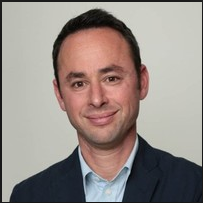
\includegraphics[width=1.86in,height=1.13in]{image1.png}
	\end{Center}
{\fontsize{10pt}{12.0pt}\selectfont \textbf{\ \ \ \ \ \ \ \ \   }} \par } & 
\multicolumn{1}{|p{4.23in}|}{{\fontsize{10pt}{12.0pt}\selectfont \textbf{Personal Information}} \par \begin{itemize}
	\item {\fontsize{10pt}{12.0pt}\selectfont Name: Sam Wick} \par 	\item {\fontsize{10pt}{12.0pt}\selectfont Job Title: Student} \par 	\item {\fontsize{10pt}{12.0pt}\selectfont Age: 26 years} \par 	\item {\fontsize{10pt}{12.0pt}\selectfont University: University of Ottawa} \par 	\item {\fontsize{10pt}{12.0pt}\selectfont Email: wicksam@gmail.com}
\end{itemize} \par } \\
\hhline{--}
%row no:2
\multicolumn{2}{|p{6.29in}|}{{\fontsize{10pt}{12.0pt}\selectfont \textbf{Skills}} \par \begin{itemize}
	\item {\fontsize{10pt}{12.0pt}\selectfont \textbf{research and data analysis} - undertaking research and applying analytical skills} \par 	\item {\fontsize{10pt}{12.0pt}\selectfont \textbf{practical skills }- planning, executing and reporting experiments, using technical equipment and paying attention to detail} \par 	\item {\fontsize{10pt}{12.0pt}\selectfont \textbf{numeracy - }skills in using mathematics to find solutions to scientific problems, mathematical modelling and interpreting and presenting information graphically}
\end{itemize} \par } \\
\hhline{--}
%row no:3
\multicolumn{2}{|p{6.29in}|}{{\fontsize{10pt}{12.0pt}\selectfont \textbf{Experience}} \par {\fontsize{10pt}{12.0pt}\selectfont Sam has a four years’ experience as a graduate student in Physics, two years as a student of Masters in physics and now he has a one year experience of PhD in physics, which he is currently pursuing. } \par } \\
\hhline{--}
%row no:4
\multicolumn{2}{|p{6.29in}|}{{\fontsize{10pt}{12.0pt}\selectfont \textbf{User requirements}} \par {\fontsize{10pt}{12.0pt}\selectfont Cloud backup of calculations, Saving results, Viewing history, Mobile application of this calculator} \par } \\
\hhline{--}
%row no:5
\multicolumn{2}{|p{6.29in}|}{{\fontsize{10pt}{12.0pt}\selectfont \textbf{Goals}} \par {\fontsize{10pt}{12.0pt}\selectfont Sam want to use the calculator in his studies mainly in the following areas:} \par {\fontsize{10pt}{12.0pt}\selectfont 1)To calculate magnetic force (2) In Biot-savarts law(3) To calculate coulomb law(4) In Samsung pie process(mobile) (5) flow of liquid in a tube (6) flow of blood in arteries} \par } \\
\hhline{--}

\end{tabular}
 \end{table}


%%%%%%%%%%%%%%%%%%%% Table No: 1 ends here %%%%%%%%%%%%%%%%%%%%


\vspace{\baselineskip}

\vspace{\baselineskip}

\vspace{\baselineskip}

\vspace{\baselineskip}

\vspace{\baselineskip}

\vspace{\baselineskip}

\vspace{\baselineskip}

\vspace{\baselineskip}

\vspace{\baselineskip}

\vspace{\baselineskip}
\begin{justify}
\textbf{PROBLEM 4 [40 MARKS]}
\end{justify}\par


\vspace{\baselineskip}

\vspace{\baselineskip}


%%%%%%%%%%%%%%%%%%%% Figure/Image No: 1 starts here %%%%%%%%%%%%%%%%%%%%

\begin{figure}[H]
	\begin{Center}
		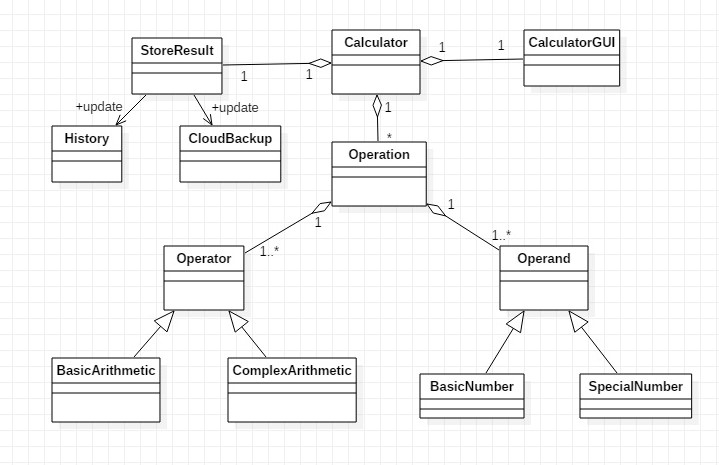
\includegraphics[width=482.25pt,height=311.75pt]{image2.jpeg}
	\end{Center}
\end{figure}


%%%%%%%%%%%%%%%%%%%% Figure/Image No: 1 Ends here %%%%%%%%%%%%%%%%%%%%

\begin{justify}
\textbf{\  }
\end{justify}\par


\vspace{\baselineskip}
\begin{Center}
\textbf{Figure 1: Problem Domain Model}
\end{Center}\par


\vspace{\baselineskip}

\vspace{\baselineskip}

\vspace{\baselineskip}

\vspace{\baselineskip}

\vspace{\baselineskip}

\vspace{\baselineskip}

\vspace{\baselineskip}

\vspace{\baselineskip}

\vspace{\baselineskip}

\vspace{\baselineskip}

\vspace{\baselineskip}

\vspace{\baselineskip}

\vspace{\baselineskip}

\vspace{\baselineskip}

\vspace{\baselineskip}
\begin{justify}
\textbf{PROBLEM 5 [50 MARKS]}
\end{justify}\par


\vspace{\baselineskip}


%%%%%%%%%%%%%%%%%%%% Figure/Image No: 2 starts here %%%%%%%%%%%%%%%%%%%%

\begin{figure}[H]
	\begin{Center}
		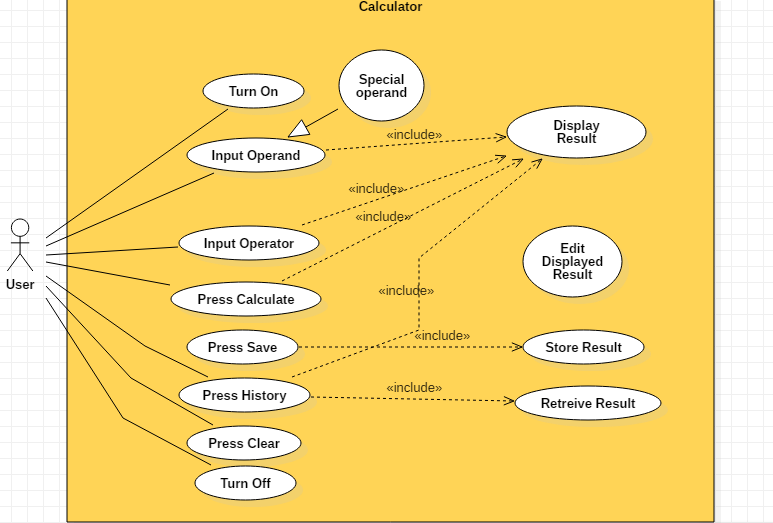
\includegraphics[width=6.5in,height=4.4in]{image3.png}
	\end{Center}
\end{figure}


%%%%%%%%%%%%%%%%%%%% Figure/Image No: 2 Ends here %%%%%%%%%%%%%%%%%%%%

\par


\vspace{\baselineskip}
\begin{Center}
\textbf{Figure 2: UML Use Case Diagram}
\end{Center}\par


\vspace{\baselineskip}

\vspace{\baselineskip}

\vspace{\baselineskip}

\vspace{\baselineskip}

\vspace{\baselineskip}

\vspace{\baselineskip}

\vspace{\baselineskip}

\vspace{\baselineskip}

\vspace{\baselineskip}

\vspace{\baselineskip}

\vspace{\baselineskip}

\vspace{\baselineskip}

\vspace{\baselineskip}

\vspace{\baselineskip}

\vspace{\baselineskip}

\vspace{\baselineskip}
\begin{justify}
\textbf{Description of some use cases: }
\end{justify}\par

\begin{justify}
\textbf{Input Operand: }The type of operands a user can enter in this calculator are normal integers or irrational numbers.
\end{justify}\par

\begin{justify}
\textbf{Input Operator: }Basic Arithmetic operators (+, -, $\ast$ , /) and some complex operators (log, $ \surd$ , x! etc.)
\end{justify}\par

\begin{justify}
\textbf{Press Calculate: }This use case acts same as an $``$=$"$  operator. It will calculate the expression displayed at the screen.
\end{justify}\par

\begin{justify}
\textbf{Press Save: }To save the result, which will then be shown in a particular order, when the user would want to see history of his calculations.
\end{justify}\par

\begin{justify}
\textbf{Press History: }To view all the $``$saved$"$  calculations in the same order in which they were done.
\end{justify}\par

\begin{justify}
\textbf{Press Clear: }To clear everything displayed on the screen to $``$0$"$ .
\end{justify}\par


\vspace{\baselineskip}

\vspace{\baselineskip}

\vspace{\baselineskip}

\vspace{\baselineskip}

\vspace{\baselineskip}

\vspace{\baselineskip}

\vspace{\baselineskip}

\vspace{\baselineskip}

\vspace{\baselineskip}

\vspace{\baselineskip}

\vspace{\baselineskip}

\vspace{\baselineskip}

\vspace{\baselineskip}

\vspace{\baselineskip}

\vspace{\baselineskip}

\vspace{\baselineskip}

\vspace{\baselineskip}

\vspace{\baselineskip}


%%%%%%%%%%%%%%%%%%%% Figure/Image No: 3 starts here %%%%%%%%%%%%%%%%%%%%

\begin{figure}[H]
	\begin{Center}
		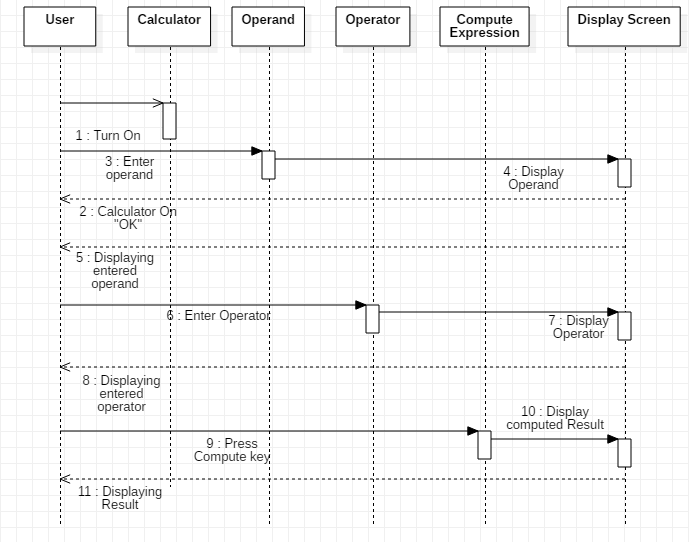
\includegraphics[width=468pt,height=368.15pt]{image4.png}
	\end{Center}
\end{figure}


%%%%%%%%%%%%%%%%%%%% Figure/Image No: 3 Ends here %%%%%%%%%%%%%%%%%%%%


\vspace{\baselineskip}

\vspace{\baselineskip}
\begin{Center}
\textbf{Figure 3: UML Sequence Diagram}
\end{Center}\par


\vspace{\baselineskip}

\vspace{\baselineskip}

\vspace{\baselineskip}

\vspace{\baselineskip}

\vspace{\baselineskip}

\vspace{\baselineskip}

\vspace{\baselineskip}

\vspace{\baselineskip}

\vspace{\baselineskip}

\vspace{\baselineskip}

\vspace{\baselineskip}

\vspace{\baselineskip}

\vspace{\baselineskip}

\vspace{\baselineskip}

\vspace{\baselineskip}
\begin{justify}
\textbf{SCENARIO TO CALCULATE CIRCUMFERENCE OF A CIRCLE (2}\textcolor[HTML]{545454}{$\ast$ }\textbf{$ \pi $ $\ast$ r)}
\end{justify}\par

\setlength{\parskip}{2.04pt}
\begin{justify}
\textbf{Step 1: }Turn on the calculator
\end{justify}\par

\begin{justify}
\textbf{Step 2: }Input Operand 2 (Basic Number)
\end{justify}\par

\begin{justify}
\textbf{Step 3: }Input Operator $\ast$  (Basic arithmetic operator)
\end{justify}\par

\begin{justify}
\textbf{Step 4: }Input Operand $ \pi $  (Special Number)
\end{justify}\par

\begin{justify}
\textbf{Step 5: }Input Operator $\ast$ 
\end{justify}\par

\begin{justify}
\textbf{Step 6: }Input Operand r (Basic Number)
\end{justify}\par

\begin{justify}
\textbf{Step 7: }Press Calculate, the expression 2$\ast$ $ \pi $ $\ast$ r will be computed
\end{justify}\par

\begin{justify}
\textbf{Step 8: }Press Save, the result of the expression 2$\ast$ $ \pi $ $\ast$ r will be saved and can be viewed by pressing history.
\end{justify}\par

\begin{justify}
\textbf{Step 9: }Press Clear, to start another computation
\end{justify}\par

\begin{justify}
\textbf{Step 10: }Turn off the calculator
\end{justify}\par


\vspace{\baselineskip}

\vspace{\baselineskip}

\vspace{\baselineskip}

\vspace{\baselineskip}

\vspace{\baselineskip}

\vspace{\baselineskip}

\vspace{\baselineskip}

\vspace{\baselineskip}

\vspace{\baselineskip}
\begin{justify}
\textbf{Glossary:}
\end{justify}\par

\begin{justify}
1. Interviewer: The person asking the questions in an interview
\end{justify}\par

\begin{justify}
2. Interviewee: The person giving answers to the interviewer
\end{justify}\par

\begin{justify}
3. Interview: A conversation between two or more people (playing the role of the interviewer and the interviewee, respectively) where questions are asked by the interviewer to obtain information from the interviewee.
\end{justify}\par

\begin{justify}
3. Persona: A fictional but realistic user of a software system.
\end{justify}\par

\begin{justify}
4. Problem Domain Model: The domain model is a representation of meaningful real-world concepts pertinent to the domain that need to be modeled in software.
\end{justify}\par

\begin{justify}
5. Use Case: In software and systems engineering, a use case is a list of actions or event steps typically defining the interactions between a role and a system to achieve a goal
\end{justify}\par


\vspace{\baselineskip}

\vspace{\baselineskip}

\vspace{\baselineskip}

\vspace{\baselineskip}

\vspace{\baselineskip}

\vspace{\baselineskip}

\vspace{\baselineskip}

\vspace{\baselineskip}

\vspace{\baselineskip}

\vspace{\baselineskip}

\vspace{\baselineskip}

\vspace{\baselineskip}

\vspace{\baselineskip}
\begin{justify}
\textbf{References: }
\end{justify}\par

\setlength{\parskip}{0.0pt}
\begin{justify}
[1] $``$What Is Pi, and How Did It Originate?$"$  by Steven Bogart 1999
\end{justify}\par

\begin{justify}
\href{https://www.scientificamerican.com/article/what-is-pi-and-how-did-it-originate/}{https://www.scientificamerican.com/article/what-is-pi-and-how-did-it-originate/}
\end{justify}\par

\begin{justify}
[2] \href{https://www.piday.org/}{https://www.piday.org/}
\end{justify}\par

\begin{justify}
[3] $``$6 THINGS YOU PROBABLY DIDN'T KNOW ABOUT PI$"$  by Rhett Allain
\end{justify}\par

\begin{justify}
\href{https://www.wired.com/2016/03/six-things-probably-didnt-know-pi/}{https://www.wired.com/2016/03/six-things-probably-didnt-know-pi/}
\end{justify}\par

\begin{justify}
[4]$"$ Wikipedia, Pi$"$ 
\end{justify}\par

\begin{justify}
 \href{https://en.wikipedia.org/wiki/Pi}{https://en.wikipedia.org/wiki/Pi$\#$ Role\_and\_characterizations\_in\_mathematics}
\end{justify}\par

\begin{justify}
[5] What Makes Pi So Special? By Natalie Wolchover
\end{justify}\par

\begin{justify}
\href{https://www.livescience.com/34132-what-makes-pi-special.html}{https://www.livescience.com/34132-what-makes-pi-special.html}
\end{justify}\par

\begin{justify}
[6] P. Kamthan, summer 2019, $``$Project Description$"$ ,
\end{justify}\par

\begin{justify}
Department of Csc. $\&$  SE, Concordia University
\end{justify}\par


\vspace{\baselineskip}

\vspace{\baselineskip}

\vspace{\baselineskip}

\vspace{\baselineskip}
\setlength{\parskip}{2.04pt}
\begin{justify}
\ \ \ \ \ \  
\end{justify}\par


\vspace{\baselineskip}

\vspace{\baselineskip}

\vspace{\baselineskip}
\setlength{\parskip}{8.04pt}

\printbibliography
\end{document}